\chapter{Ondas eletromagnéticas}
\textsl{{\sffamily(Versão: \today)}}

\noindent
Começamos agora o estudo da luz propriamente dita, descrevendo-a como uma
perturbação autoinduzida dos campos elétricos e magnéticos no espaço, regida
pelas leis fundamentais do eletromagnetismo, as equações de Maxwell.

Antes, porém, faz-se uma revisão rápida dos produtos escalar e vetorial de
vetores e dos operadores diferenciais necessários para esse estudo.

\section{Preâmbulo matemático}
\subsection{Produto escalar e produto vetorial de vetores}
Dados dois vetores, define-se o seu \emph{produto escalar} (ou \emph{produto
interno}) como o escalar que se obtém multiplicando os módulos dos dois vetores
e o cosseno do ângulo entre eles. Assim, se $\vec a$ e $\vec b$ forem os dois
vetores e $\theta$ for o ângulo que definem, o produto escalar
é\footnote{Nestes apontamentos usa-se uma convenção tipográfica usual em física,
  em que se representa o módulo de um vetor $\vec a$ por $a$: a mesma letra, mas
sem a setinha por cima.}
\begin{equation}
  \vec a\cdot\vec b= ab\cos\theta.
\end{equation}
É imediato verificar que o produto escalar de dois vetores pode ser positivo (se
o ângulo entre eles for menor que 90\deg), negativo (se for maior que 90\deg) ou
nulo (se os dois vetores forem perpendiculares). Verifica-se também
que este produto é comutativo, isto é, $\vec a\cdot\vec b=\vec b\cdot\vec a$.


Sejam respetivamente $(a_x,\,a_y,\,a_z)$ e $(b_x,\,b_y,\,b_z)$ as componentes
dos vetores $\vec a$ e $\vec b$ relativamente a alguma base ortonormada
pré-escolhida, formada por versores (vetores com norma 1) $\he_x$, $\he_y$ e
$\he_z$. Isto quer dizer que estes dois vetores se podem escrever como as
combinações lineares dos vetores da base seguintes
\begin{align*}
  \vec a&=a_x\he_x+a_y\he_y+a_z\he_z&
  \vec b&=b_x\he_x+b_y\he_y+b_z\he_z.
\end{align*}
O produto escalar destes dois vetores pode então desenvolver-se como
\begin{align*}
  \vec a\cdot\vec b&=
  (a_x\he_x+a_y\he_y+a_z\he_z) \cdot (b_x\he_x+b_y\he_y+b_z\he_z)\\
  &=a_xb_x(\he_x\cdot\he_x)+ a_xb_y(\he_x\cdot\he_y)+ a_xb_z(\he_x\cdot\he_z)\\
  &+a_yb_x(\he_y\cdot\he_x)+ a_yb_y(\he_y\cdot\he_y)+ a_yb_z(\he_y\cdot\he_z)\\
  &+a_zb_x(\he_z\cdot\he_x)+ a_zb_y(\he_z\cdot\he_y)+ a_zb_z(\he_z\cdot\he_z)
\end{align*}
Mas os produtos escalares de versores da base diferentes são nulos (porque eles
são todos perpendicuares entre si) e os produtos escalares de um qualquer versor
da base consigo próprio é 1 (porque o módulo dos versores é 1 e o cosseno do
ângulo [nulo] que um vetor faz consigo próprio também é 1), isto é,
\begin{align*}
  \he_x\cdot\he_x=\he_y\cdot\he_y=\he_z\cdot\he_z=1\\
  \he_x\cdot\he_y=\he_y\cdot\he_z=\he_z\cdot\he_x=0.
\end{align*}
Substituindo em cima, obtemos uma forma alternativa para o produto escalar de
dois vetores:
\begin{equation}
  \vec a\cdot\vec b=a_xb_x+a_yb_y+a_zb_z.
\end{equation}

Define-se também o \emph{produto vetorial} ou \emph{produto externo} de vetores.
Como o próprio nome indica, o produto vetorial de dois vetores é ainda um
vetor\footnote{Ao contrário do produto escalar de vetores que, como acabámos de
ver, é... Um escalar.}. A norma do produto escalar de dois vetores é o produto
das suas normas e do seno do ângulo entre eles:
\begin{equation}
  \|\vec a\times\vec b\|=ab\sin\theta;
\end{equation}
a sua direção é a perpendicular ao plano definido pelos dois vetores que se
multiplicam e o sentido é o definido pela regra da mão direita\footnote{%
  \parbox[t]{0.8\textwidth}{Há várias formas de enunciar esta regra, pode
    encontrá-las todas rapidamente numa pesquisa na web (experimente usar
    ``cross product right hand rule'' como expressão de busca). Escolha a que
    preferir. Eu gosto desta: oriente o indicador da mão direita como o primeiro
    vetor no produto e o médio da mesma mão como o segundo; o polegar indica
  então o sentido do produto vetorial (veja a figura ao lado, retirada da
  Wikipedia)}\hfill
  \parbox[t]{1.8cm}{%
    \raisebox{-0.8\height}{%
      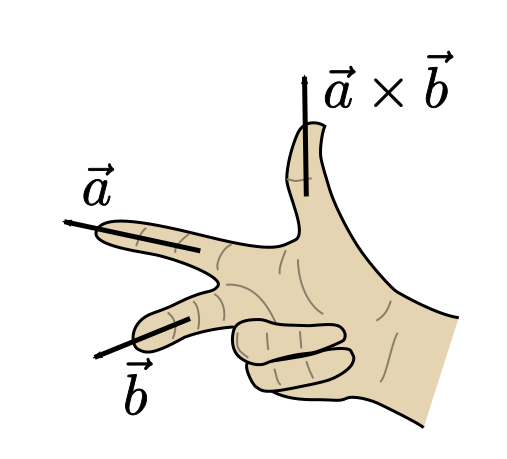
\includegraphics[width=1.7cm]{sections/02emw/figs/rhr.png}
    }
  }
}.
O produto vetorial assim definido é \emph{anticomutativo}, isto é, o sinal do
resultado é trocado se trocarmos a ordem dos fatores: $\vec a\times\vec b=-\vec
b\times\vec a$. Constata-se também que
\begin{align}
  \he_x\times\he_y&=\he_z&
  \he_y\times\he_z&=\he_x&
  \he_z\times\he_x&=\he_y.
\end{align}
Munidos destas igualdades (e das que resultam trocando a ordem dos fatores nos
seus lados esquerdos) obtemos uma expressão para o cálculo do vetor produto
vetorial em termos das componentes dos dois vetores multipicados externamente.
Sejam, como há pouco, $a_x,\,a_y,\,a_z$ e $b_x,\,b_y,\,b_z$ as componentes de
dois vetores $\vec a $ e $\vec b$ relativamente a uma base ortonormada formada
por vetores unitarios $\he_x$ $\he_y$, $\he_z$. Então,
\begin{equation*}
  \vec a = a_x\he_x+a_y\he_y+a_z\he_z\rule{2cm}{0mm}
  \vec b = b_x\he_x+b_y\he_y+b_z\he_z,
\end{equation*}
e, assim,
\begin{align*}
  \vec a \times \vec b &=
  (a_x\he_x+a_y\he_y+a_z\he_z)\times
  (b_x\he_x+b_y\he_y+b_z\he_z)\\
  &=
  (a_yb_z-a_zb_y)\he_x+(a_zb_x-a_xb_z)\he_y+(a_xb_y-a_yb_x)\he_z.
\end{align*}
Esta expressão para o produto vetorial de dois vetores em termos das componentes
dos vetores multiplicados é fácil de memorizar notando que pode também ser vista
como o determinante da matriz simbólica (verifique):
\begin{equation}
  \vec a\times\vec b =\det
  \begin{bmatrix}
    \he_x&\he_y&\he_z\\
    a_x&a_y&a_z\\
    b_x&b_y&b_z
  \end{bmatrix}.
\end{equation}

\subsection{Operadores diferenciais}
As equações de Maxwell são quatro equações às derivadas parciais dos campos
elétrico e magnético que traduzem localmente\footnote{Isto é, como igualdades
que relacionam o valor de funções em cada ponto do espaço.} as leis integrais
do eletromagnetismo que foram estudadas na cadeira de Física Geral II, a saber:
a lei de Gauss do campo elétrico (e uma que desempenha um papel semelhante para
o campo magnético), a lei de Faraday e a lei de Ampère. Estas equações envolvem
os operadores diferenciais divergência e rotacional, que vamos agora,
rapidamente, recordar.

\subsection*{Divergência de um campo vetorial}
A divergência de um campo vetorial é um escalar igual ao fluxo do campo por
unidade de volume.  De um modo talvez mais intuitivo (mas muito menos preciso),
podemos dizer que é a \emph{``quantidade'' de campo que ``sai''} desse ponto por
unidade de volume.  

Pode demonstrar-se (mas não o faremos aqui) que, usando
coordenadas cartesianas, a divergência de um campo vetorial $\vec V$ é dada por
\begin{equation}\label{eq:divcart}
  \div\vec V=\pd{V_x}{x} + \pd{V_y}{y}+\pd{V_z}{z}.
\end{equation}
Introduzindo agora o símbolo vetorial ``nabla'' 
\begin{equation*}
  \vec \nabla = (\pd{}{x},\, \pd{}{y},\, \pd{}{z}),
\end{equation*}
a divergência de $\vec V$ pode ainda escrever-se de forma mais condensada como
o produto escalar de nabla e $\vec V$:
\begin{equation}
  \div\vec V=\vec\nabla\cdot\vec V.
\end{equation}


\subsection*{Rotacional de um campo vetorial}
O rotacional de um campo vetorial é um vetor igual à circulação do campo por
unidade de área. A sua direção é a perpendicular ao plano onde a circulação tem
o valor máximo. Em termos intuitivos (mas terivelmente imprecisos), o rotacional
dá uma ideia de \emph{``quanto'' é que o campo ``roda''} num ponto; a sua
direção é do ``eixo'' dessa ``rotação'' e o sentido é o dado pela regra da mão
direita a partir do sentido da ``rotação'' do campo. 

O rotacional de um campo $\vec V$ é, em coordenadas cartesianas, dado por
\begin{equation}\label{eq:rotcart}
  \rot\vec V=
  \left(\pd{V_z}{y}-\pd{V_y}{z},\; \pd{V_x}{z}-\pd{V_z}{x},\;
  \pd{V_y}{x}-\pd{V_x}{y}\right).
\end{equation}
Em termos do símbolo vetorial nabla, fica, mais sucintamente,
\begin{equation}
  \rot\vec V=\vec\nabla\times\vec V.
\end{equation}

{\small%
  Feita esta abreviadíssima explicação sobre os operadores $\div$ e $\rot$,
  talvez não seja pior referir alguns factos mais básicos da ``vida secreta
  das derivadas''. Uma função crescente tem uma variação positiva quando a
  variável de que depende sofre um acréscimo; logo, a sua taxa de variação
  (variação da função a dividir pelo acréscimo da variável) é positiva, logo a
  sua derivada (outro nome para a taxa de variação) é positiva. Do mesmo modo,
  uma função decrescente tem derivada negativa. Uma função constante não é
  crescente nem decrescente; logo, não tem derivada positiva nem negativa, tem
  derivada nula.  Uma função que atinge um valor extremo (máximo ou mínimo) para
  um dado valor da variável de que depende, nesse ponto não é crescente nem
  decrescente: tem derivada nula nesse ponto.

  Quando estudamos funções de várias variáveis (como é o caso agora), estas
  regras ainda se aplicam mas têm que ser consideradas com cuidado porque a
  função pode ser crescente relativamente aos acréscimos de uma variável,
  decrescente com acréscimos de outra variável e constante com acréscimos de uma
  terceira variável. Assim, uma função que depende da posição e do tempo e que
  num dado ponto tem um valor que vai paulatinamente aumentando à medida que o
  tempo passa, é uma função que tem, nesse ponto, derivada temporal positiva. Se
  o seu valor num dado ponto se mantém inalterado com a passagem do tempo, então
  a sua derivada temporal, nesse ponto, é nula. E etc, etc, etc, acho que destes
  dois exemplos já se vai percebendo a lógica geral.

  A derivada de uma função de várias variáveis em ordem a uma delas é ainda, em
  geral, uma função dessas mesmas variáveis. Como tal, pode fazer sentido
  derivá-la novamente, em ordem à mesma variável ou em ordem a outra qualquer. O
  teorema de Swartz garante que esta derivada não depende da ordem com que se
  fazem cada uma das derivações:
  \begin{equation*}
    \cpdd{f}{x}{y}=
    \cpdd{f}{y}{x},\qquad\text{Qualquer que seja a função $f$}
  \end{equation*}
}

\section{Equações de Maxwell}
As quatro equações de Maxwell para os campos elétrico ($\vec E$) e magnético
($\vec B$) são as seguintes:
\begin{align*}
  \div\vec E&=\frac{\rho}{\epsilon_0}&\div\vec B&=0\\
  \rot\vec E&=-\pd{\vec B}{t}&
  \rot\vec B&=\mu_0\vec j+\mu_0\epsilon_0\pd{\vec E}{t}.
\end{align*}
Nestas expressões, $\epsilon_0=\simeq8,8542\times10^{-12}$\,F/m representa a
permitividade elétrica do vácuo, $\mu_0=4\pi\times10^{-7}$\,H/m a permeabilidade
magnética do vácuo, $\rho$ a densidade de carga (carga por unidade de volume)
total em cada ponto e $\vec j$ a densidade de corrente (corrente elétrica por
unidade de área) total em cada ponto.

Interessam-nos particularmente nestes apontamentos campos variáveis em locais
afastados de cargas e correntes (que constituem, veremos, ondas eletromagnéticas
afastadas das suas fontes). Por isso vamos considerar, para já pelo menos, a
densidade de carga $\rho$ e a densidade de corrente $\vec j$ ambas nulas. As
equações de Maxwell assumem então a forma, mais simétrica, que iremos, quase
sempre, considerar nesta disciplina,\footnote{Para falicitar a referência,
  ordenamos aqui estas equações em ordem crescente da esquerda para a direita e
  de cima para baixo. Assim, chamremos ``primeira equação de Maxwell'' à que
  apresenta a divergência do campo elétrico (lei de Gauss), ``terceira equação
  de Maxwell'' à que envolve o rotacional do mesmo campo (lei de Faraday), etc.}
\begin{equation}\label{eq:meqs}
  \begin{aligned}
    \div\vec E&=0& \div\vec B&=0\\
    \rot\vec E&=-\pd{\vec B}{t}& \qquad\qquad
      \rot\vec B&=\mu_0\epsilon_0\pd{\vec E}{t}.
  \end{aligned}
\end{equation}

Procuremos soluções destas equações. A mais simples de todas é a trivial:
\begin{align*}
  \vec E&=0&\vec B=0.
\end{align*}
É pouco interessante, convenhamos. A seguir, em ordem crescente de complexidade,
consideremos um campo eletromagnético constante e uniforme, isto um campo
elétrico que tem em todos os pontos a mesma intensidade e orientação e que
mantêm essas características inalteradas em todos os instantes, e o mesmo para o
campo magnético. Estes campos têm derivadas todas nulas em todos os pontos e em
todos os instantes e, assim, são também solução das equações de Maxwell. Mas há
uma certa quantidade de energia associada ao campo, e um campo uniforme (ou
seja, definido em todo o espaço com uma mesma intensidade e orientação) tem uma
energia infinita. São, assim, soluções não realistas das equações de
Maxwell e por isso não a consideraremos (excepto se $\vec E$ e $\vec B$ forem
constante e uniformemente nulos, caso que já tratámos). Resumindo:

Consideremos agora o caso dos campos que dependem de ponto para ponto, mas são
constantes (independentes do tempo). Suponhamos, por exemplo, que o campo
magnético $\vec B$ é constante, mas apresenta valores e/ou orientações
diferentes de ponto para ponto. Então $\partial \vec B/\partial t=0$; a terceira
equação de Maxwell mostra então que $\rot \vec E=0$. Mas um campo com
divergência nula e com rotacional nulo é um campo com todas as derivadas
espaciais nulas, ou seja, um campo uniforme. Concluímos que $\vec E$ é uniforme
e, pelas razões atrás apresentadas, só pode ser nulo em todo o espaço,
constantemente nulo, entenda-se. Então a derivada $\partial \vec E/\partial t$
anula-se; logo, de acordo com a última das equações, $\rot \vec B=0$: o campo
magnético, afinal, tem as derivadas espaciais todas nulas! Logo, é uniforme e,
portanto, como vimos no parágrafo anterior, só pode ser nulo.

\section{Ondas eletromagnéticas}
Verificámos que campos uniformes e constantes só podem ser nulos, que campos
constantes (mesmo que não sejam uniformes) também só podem ser nulos, e
poderíamos verificar (tente fazê\-\mbox{-lo}!) que campos uniformes (mesmo que não sejam
constantes) também devem anular-se. Ou seja, que soluções constantes e/ou
uniformes constituem, na realidade, a solução trivial $\vec E=\vec B=0$.
Vamos agora considerar situações mais interessantes, em que os campos dependem da
posição \emph{e} do tempo.

\subsection*{Um caso particular ilustrativo}
Mantendo a situação o mais simples possível, consideremos um campo elétrico que
depende do tempo e de apenas uma coordenada espacial, que escolhemos ser a
coordenada $x$,
\begin{equation*}
  \vec E=\vec E(x,t).
\end{equation*}
Como o campo (as três componentes do campo) só dependem de $t$ e de $x$, as suas
derivadas relativamente às outras coordenadas $y$ e $z$ são nulas, isto é,
\begin{align*}
  \pd{\vec E}{y}=\pd{\vec E}{z}=0,
\end{align*}
e repare que afirmar que as derivadas do vetor campo elétrico se anulam
significa dizer que se anulam as derivadas \emph{de cada componente} do campo
elétrico.

Tendo em conta a expressão da divergência de um campo vetorial da
\eqref{eq:divcart}, a primeira das equações de Mawell pode também escrever-se
como
\begin{equation*}
  \pd{E_x}{x}+\pd{E_y}{y}+\pd{E_z}{z}=0,
\end{equation*}
que, de acordo com o que acabámos de discutir, se reduz neste caso em que o
campo só depende da coordenada $x$ a
\begin{equation*}
  \pd{E_x}{x}=0,
\end{equation*}
ou seja, a componente $x$ do campo é uniforme. Mas então, como vimos na secção
anterior, deve ser nula, $E_x=0$. Estes argumentos podem ser aplicados sem
alteração para o campo magnético, ou considerando campos que dependem apenas da
coordenada $y$ ou $z$. Podemos assim concluir que se o campo elétrico ou o campo
magnético dependem apenas de uma das coordenadas, então a componente
correspondente a essa coordenada é nula.

Dado que $E_x=0$ e que $\partial E_\alpha/\partial y=\partial E_\alpha/\partial
z=0$ (qualquer que seja a componente $E_\alpha$ do campo), as equações para o
rotacional dos campos elétrico e magnético (na segunda linha das
eqs.~\eqref{eq:meqs}), tendo em conta a expressão do rotacional em coordenadas
cartesianas da eq.~\eqref{eq:rotcart}, podem escrever-se como
\begin{subequations}
\begin{align}
  0&=-\pd{B_x}{t}&        \pd{B_z}{y}-\pd{B_y}z&=0\label{eq:meqx}\\
  \pd{E_z}{x}&=\pd{B_y}{t}&  \pd{B_x}{z}-\pd{B_z}{x}&=
    \epsilon_0\mu_0\pd{E_y}{t} \label{eq:meqy}\\
  \pd{E_y}{x}&=-\pd{B_z}{t}& 
    \pd{B_y}{x}-\pd{B_y}{x}&=\epsilon_0\mu_0\pd{E_z}{t}\label{eq:meqz}
\end{align}
\end{subequations}
Tomemos a igualdade no lado esquerdo da eq.~\eqref{eq:meqy} e derivêmo-la em
ordem a $x$. Resulta
\begin{equation*}
  \pdd{E_z}{x}=\pd{}{t}\pd{B_y}{x}.
\end{equation*}
Mas a igualdade no lado direito da eq.~\eqref{eq:meqy} pode escrever-se como
\begin{equation*}
  \pd{B_y}{x}=\pd{B_y}{x}+\epsilon_0\mu_0\pd{E_z}{t}.
\end{equation*}
Substituindo em cima, obtemos
\begin{equation*}
  \pdd{E_z}{x}=\pd{}{t}\pd{B_y}{x}+\epsilon_0\mu_0\pdd{E_z}{t}
\end{equation*}
O primeiro termo no lado direito desta igualdade é nulo:
\begin{equation*}
  \pd{}{t}\pd{B_y}{x}=\pd{}{x}\pd{B_y}{t}=0,
\end{equation*}
de acordo com a equação no lado esquerdo da primeira linha. Obtemos então, por
fim,
\begin{equation*}
  \pdd{E_z}{x}=\epsilon_0\mu_0\pdd{E_z}{t}.
\end{equation*}
Mas repare-se que esta é a equação diferencial satisfeita em geral por ondas que
se propagam ao longo do eixo dos $x$ sem alteração de forma (veja a
eq.~\eqref{eq:waveq}), com velocidade
$v=1/\sqrt{\mu_0\epsilon_0}=3,00\times10^{8}$\,m/s.  Verificamos assim que as
equações de Maxwell admitem soluções que representam ondas que se propagam sem
alteração de forma com a velocidade da luz. Nesta análise, constatámos também que a
componente $x$ do campo elétrico é nula. Mas a direção do eixo dos $x$ é a
direção de propagação.  Assim, constatamos que o campo elétrico, neste exemplo,
é transversal. Veremos que se trata de uma propriedade geral do campo elétrico
(e também do magnético) numa onda eletromagnética.

\subsection{Análise mais geral}
Depois de apresentado o exemplo anterior, vejamos isto com maior generalidade.
Calculemos o rotacional da terceira equação de Maxwell, na linha de baixo e à
esquerda na eq.~\eqref{eq:meqs}:
\begin{equation*}
  \rot\rot\vec E=-\rot\pd{\vec B}{t}=-\pd{}{t}\rot\vec B.
\end{equation*}
Mas o rotacional do campo magnético é dado pela quarta equação de Maxwell.
Substibuindo aqui, obtemos
\begin{equation*}
  \rot\rot\vec E=-\epsilon_0\mu_0\pdd{\vec E}{t}.
\end{equation*}
O rotacional duplo do lado esquerdo desta igualdade pode simplificar-se
aplicando um teorema da análise de funções de várias variáveis segundo o qual
para qualquer função vetorial $\vec A$ se tem
\begin{equation*}
  \rot\rot\vec A=\grad\div\vec A - \lap\vec A.
\end{equation*}
No caso que estudamos, o primeiro termo é nulo porque, de acordo com a primeira
equação de Maxwell, $\div \vec E=0$. Resulta então, por fim,
\begin{equation}\label{eq:efplw}
  \lap\vec E=\epsilon_0\mu_0\pdd{\vec E}{t}.
\end{equation}
Mas esta é a equação geral das ondas planas em três dimensões, que deduzimos no
capítulo anterior (veja a eq.~\eqref{eq:plweq3d}). Concluímos assim, com toda a
generalidade que o campo elétrico pode existir no vazio em configurações não
triviais, na forma de ondas planas que se propagam à velocidade da luz
$c=1/\sqrt{\epsilon_0\mu_0}$ sem alteração de forma.

Poderíamos ter começado por calcular o rotacional da quarta equação de Maxwell.
Chegaríamos a uma equação semelhante à eq.~\eqref{eq:efplw} mas envolvendo agora
o campo magnético.

Agora que sabemos que há soluções das equações de Maxwell que satisfazem a
equação de onda, podemos descrever o campo elétrico (e o campo magnético também) 
com as fuções de onda harmónicas, que já vimos serem soluções da dita equação de
onda. Assim, seja o campo elétrico dado por
\begin{equation}\label{eq:hpwef}
  \vec E(\vec r,t)=\vec E_0\,\e^{\iu(\vec k\cdot\vec r-\omega t+\phi_0)}.
\end{equation}
Nesta expressão, os símbolos $\vec k$, $\omega$ e $\phi_0$ têm o significado que
já lhes atribuímos no capítulo anterior\footnote{$\vec k$ é o vetor de onda, com
  a direção e o sentido da propagação e com módulo $k=2\pi/\lambda$,
$\omega=2\pi/T$ é a frequência angular da onda e $\phi_0$ é a constante de
fase.}, mas na amplitude amplitude ($\vec E_0$) talvez se estranhe o caráter
vetorial explicitado pela setinha. Bem, como discutimos no primeiro capítulo, a
amplitude de uma onda harmónica tem a natureza da função de onda, tanto quanto
às dimensões e unidades, como quanto ao caráter escalar/vetorial. Como a função
de onda é o campo elétrico e como este é um vetor, a amplitude desta onda
harmónica é igualmente um vetor. Chama-se \emph{direção de polarização} da onda
à direção do vetor amplitude dessa onda.

Vamos agora estudar as propriedades desta onda de campo elétrico, analisando-a à
luz das equações de Maxwell. Antes, porém, vejamos como atuam os operadores
diferenciais numa função de onda como a da eq.~\eqref{eq:hpwef}. Ao mesmo tempo
que facilitará a análise que vamos fazer a seguir, este estudo revelará as
vantagens da forma exponencial complexa sobre as formas trignométricas.

Note que a expressão $\vec k\cdot\vec r$ é o produto escalar do vetor de onda
$\vec k$, com componentes $(k_x,\,k_y,\,k_z)$ e do vetor posição
$\vec r=(x,\,y,\,z)$. Assim, $\vec k\cdot\vec r=k_xx+k_yy+k_zz$;
logo,
\begin{align*}
  \pd{}{x}\e^{\iu(\vec k\cdot\vec r-\omega t+\phi_0)}&=
  \iu k_x\e^{\iu(\vec k\cdot\vec r-\omega t+\phi_0)}
\end{align*}
e, do mesmo modo,
\begin{align*}
  \pd{}{y}\e^{\iu(\vec k\cdot\vec r-\omega t+\phi_0)}&=
  \iu k_y\e^{\iu(\vec k\cdot\vec r-\omega t+\phi_0)}&
  \pd{}{z}\e^{\iu(\vec k\cdot\vec r-\omega t+\phi_0)}&=
  \iu k_z\e^{\iu(\vec k\cdot\vec r-\omega t+\phi_0)}
\end{align*}
As derivadas do campo elétrico da eq.~\eqref{eq:hpwef} são, então, dadas por
expressões simples. Por exemplo, a derivada em ordem a $x$ fica
\begin{equation*}
  \pd{}{x}\vec E=\vec E_0\pd{}{x}\e^{\iu(\vec k\cdot\vec r-\omega t+\phi_0)}=
  \iu k_x\vec E_0\e^{\iu(\vec k\cdot\vec r-\omega t+\phi_0)}=
  \iu k_x \vec E.
\end{equation*}
Expressões semelhantes obtêm-se para as restantes derivadas. Em resumo,
\begin{align*}
  \pd{\vec E}{x}&=\iu k_x\vec E&
  \pd{\vec E}{y}&=\iu k_y\vec E&
  \pd{\vec E}{z}&=\iu k_z\vec E&
  \pd{\vec E}{t}&=-\iu \omega\vec E.
\end{align*}
Essencialmente, é a simplicidade destas expressões que torna a representação das
funções harmónicas com exponenciais complexas vantajosa. Se mantivessemos a
representação com funções trignométricas, o cálculo das derivadas parciais da
função de onda seria muito mais complexo\footnote{Mas é um bom exercício
fazê-lo.  Força!}.

\subsection{As ondas eletromagnéticas são ondas transversais}
De acordo com a primeira equação de Maxwell, a divergência do campo elétrico é
nula. Mas, dada a expressão geral da divergência em coordenadas cartesianas 
(eq.~\eqref{eq:divcart}) e as igualdades que acabámos de demonstrar, temos
\begin{align*}
  \div\vec E&=\pd{E_x}{x}+\pd{E_y}{y}+\pd{E_z}{z}\\
            &=\iu k_x E_x+\iu k_y E_y+\iu k_z E_z=\iu\vec k\cdot\vec E.
\end{align*}
Se a divergência do campo é nula, é nulo o produto escalar do campo com o vetor
de onda $\vec k$. Logo, o campo elétrico é perpendicular ao vetor de onda, ou
seja, é perpendicular à direção de propagação.

Consideremos agora a terceira equação de Maxwell:
\begin{align*}
  \pd{\vec B}{t}&=-\rot\vec E\\
                &=-\rot \vec E_0\e^{\iu(\vec k\cdot\vec r-\omega t+\phi_0)}
  =-\vec \nabla\times\vec E_0\e^{\iu(\vec k\cdot\vec r-\omega t+\phi_0)}\\
  &=-\iu\vec k\times\vec E_0\e^{\iu(\vec k\cdot\vec r-\omega t+\phi_0)}.
\end{align*}
Então o campo magnético pode obter-se primitivando em ordem ao tempo o lado
direito, ou seja,
\begin{align}
  \vec B&=-\iu\vec k\times\vec E_0\int\e^{\iu(\vec k\cdot\vec r-\omega
          t+\phi_0)}dt\nonumber\\
          &=-\iu\vec k\times\vec E_0\frac{1}{-i\omega}
            \e^{\iu(\vec k\cdot\vec r-\omega t+\phi_0)}\nonumber\\
            \vec B&=\frac{1}{\omega}\vec k\times \vec E.\label{eq:mf}
\end{align}
Vemos assim que o campo magnético associado a uma onda plana eletromagnética é
proporcional ao produto vetorial do vetor de onda com o campo. Ou seja,
é perpendicular ao campo elétrico e também à direção de propagação: numa onda
eletromagnética plana, ambos os campos são transversais, e são perpendiculares
entre si. 

De acordo com a eq.~\eqref{eq:mf}, o campo magnético pode escrever-se como
\begin{equation*}
  \vec B=\vec B_0\,\e^{\iu(\vec k\cdot\vec r-\omega t+\phi_0)},\qquad
  \text{ com } 
  \vec B_0=\frac{1}{\omega}\vec k\times\vec E_0.
\end{equation*}
Este resultado mostra que o campo magnético constitui também uma onda plana
harmónica, com a mesma direção de propagação, a mesma frequência e o mesmo
comprimento que o campo elétrico, e com a mesma fase também. Para além disso, os
módulos das amplitudes do campo magnético e do campo elétrico estão também
relacionados. Uma vez que $\vec E_0$ e $\vec k$ são perpendiculares, o módulo do
produto vetorial é igual ao produto dos módulos dos dois vetores e, assim,
\begin{equation}
  B_0 = \frac{k}{\omega}E_0=\frac{E_0}{c},
\end{equation}
onde $c$ representa a velocidade de propagação da onda.

A Figura~\ref{fig:plemwave} ilustra a orientação relativa do campo elétrico, do
campo magnético e da direção de propagação, para uma direção de polarização
coincidente com o eixo dos $y$.
\begin{figure}[htb]
  {\centering
      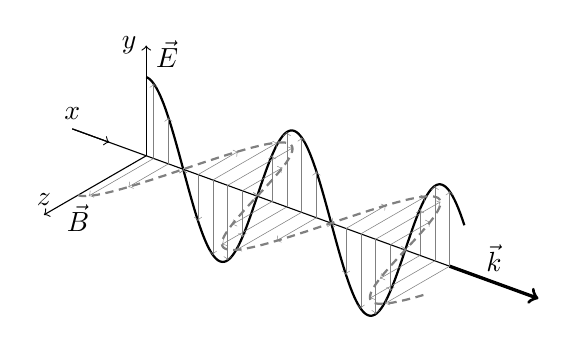
\begin{tikzpicture}[x={(-20:1cm)},y={(90:1cm)},z={(210:1cm)}]
        % Axes
        \draw (-1,0,0) node[above] {$x$} -- (5,0,0);
        \draw [->] (-1,0,0) -- (-0.5,0,0);
        \draw [->](0,0,0) -- (0,1.4,0) node[left] {$y$};
        \draw [->] (0,0,0) -- (0,0,1.5) node[above] {$z$};
        % Propagation
        \draw[->,very thick] (4.1,0,0) -- node[above] {$\vec k$} (5.3,0,0);
        % Waves
        \draw[thick] plot[domain=0:4.3,samples=200] (\x,{cos(deg(pi*\x))},0);
        \draw[gray,thick, densely dashed] plot[domain=0:4.3,samples=200]
        (\x,0,{cos(deg(pi*\x))});
        % Arrows
        \foreach \x in {0.1,0.3,...,4.2} {
          \draw[->,help lines] (\x,0,0) -- (\x,{cos(deg(pi*\x))},0);
          \draw[->,help lines] (\x,0,0) -- (\x,0,{cos(deg(pi*\x))});
        }
        % Labels
        \node[above right] at (0,1,0) {$\vec{E}$};
        \node[below] at (0,0,1) {$\vec{B}$};
      \end{tikzpicture}\par
    }
    \caption{Onda eletromagnética plana e harmónica que se propaga no sentido
    positivo do eixo dos $x$, com direção de polarização (a direção do campo
  elétrico) segundo o eixo dos $y$ e campo magnético paralelo ao eixo dos $z$.
  (Adaptado de um artigo no \LaTeX{} StackExchange.)\label{fig:plemwave}}
\end{figure}

\section{O vetor de Poynting e a irradiância}
\begin{equation*}
  \vec S=\frac{1}{\mu_0}\vec E\times\vec B.
\end{equation*}
\tobedone{}

\section{Polarização}
\tobedone{}

\section{Fotões}
\tobedone{}

\section{O espetro eletromagnético}
\tobedone{}



